
\section{Usage scenarios}\label{sec:usage-scenarios}

In addition to evaluating 1D slices with a low-level task hierarchy, we also
provide usage scenarios to understand their value in real-world applications.
We begin with an illustrative example using the 2D sinc
function.
%\ttwnote{cite?}.  TM: No need to cite!
We then use our 1D slices approach to illustrate how
it can help better understand neural network architectures for a regression
problem. Finally, we use 1D slices to investigate the effect of initial
position on optimization algorithm performance.

The purpose of these evaluations is a proof of concept that 1D slices can be
used for real-world problems. In particular, it is not meant as a comparative
evaluation as provided in the previous section. To the best of our knowledge,
neither HyperSlices nor topological techniques have been applied to
understanding neural networks nor optimization algorithms so far. A full
adaption of, and comparison to, these techniques for the provided use cases are
beyond the scope of this paper, and are left for future work. 

\subsection{2D sinc function}

\begin{figure}
  \centering
  \begin{subfigure}[b]{0.3\linewidth}
    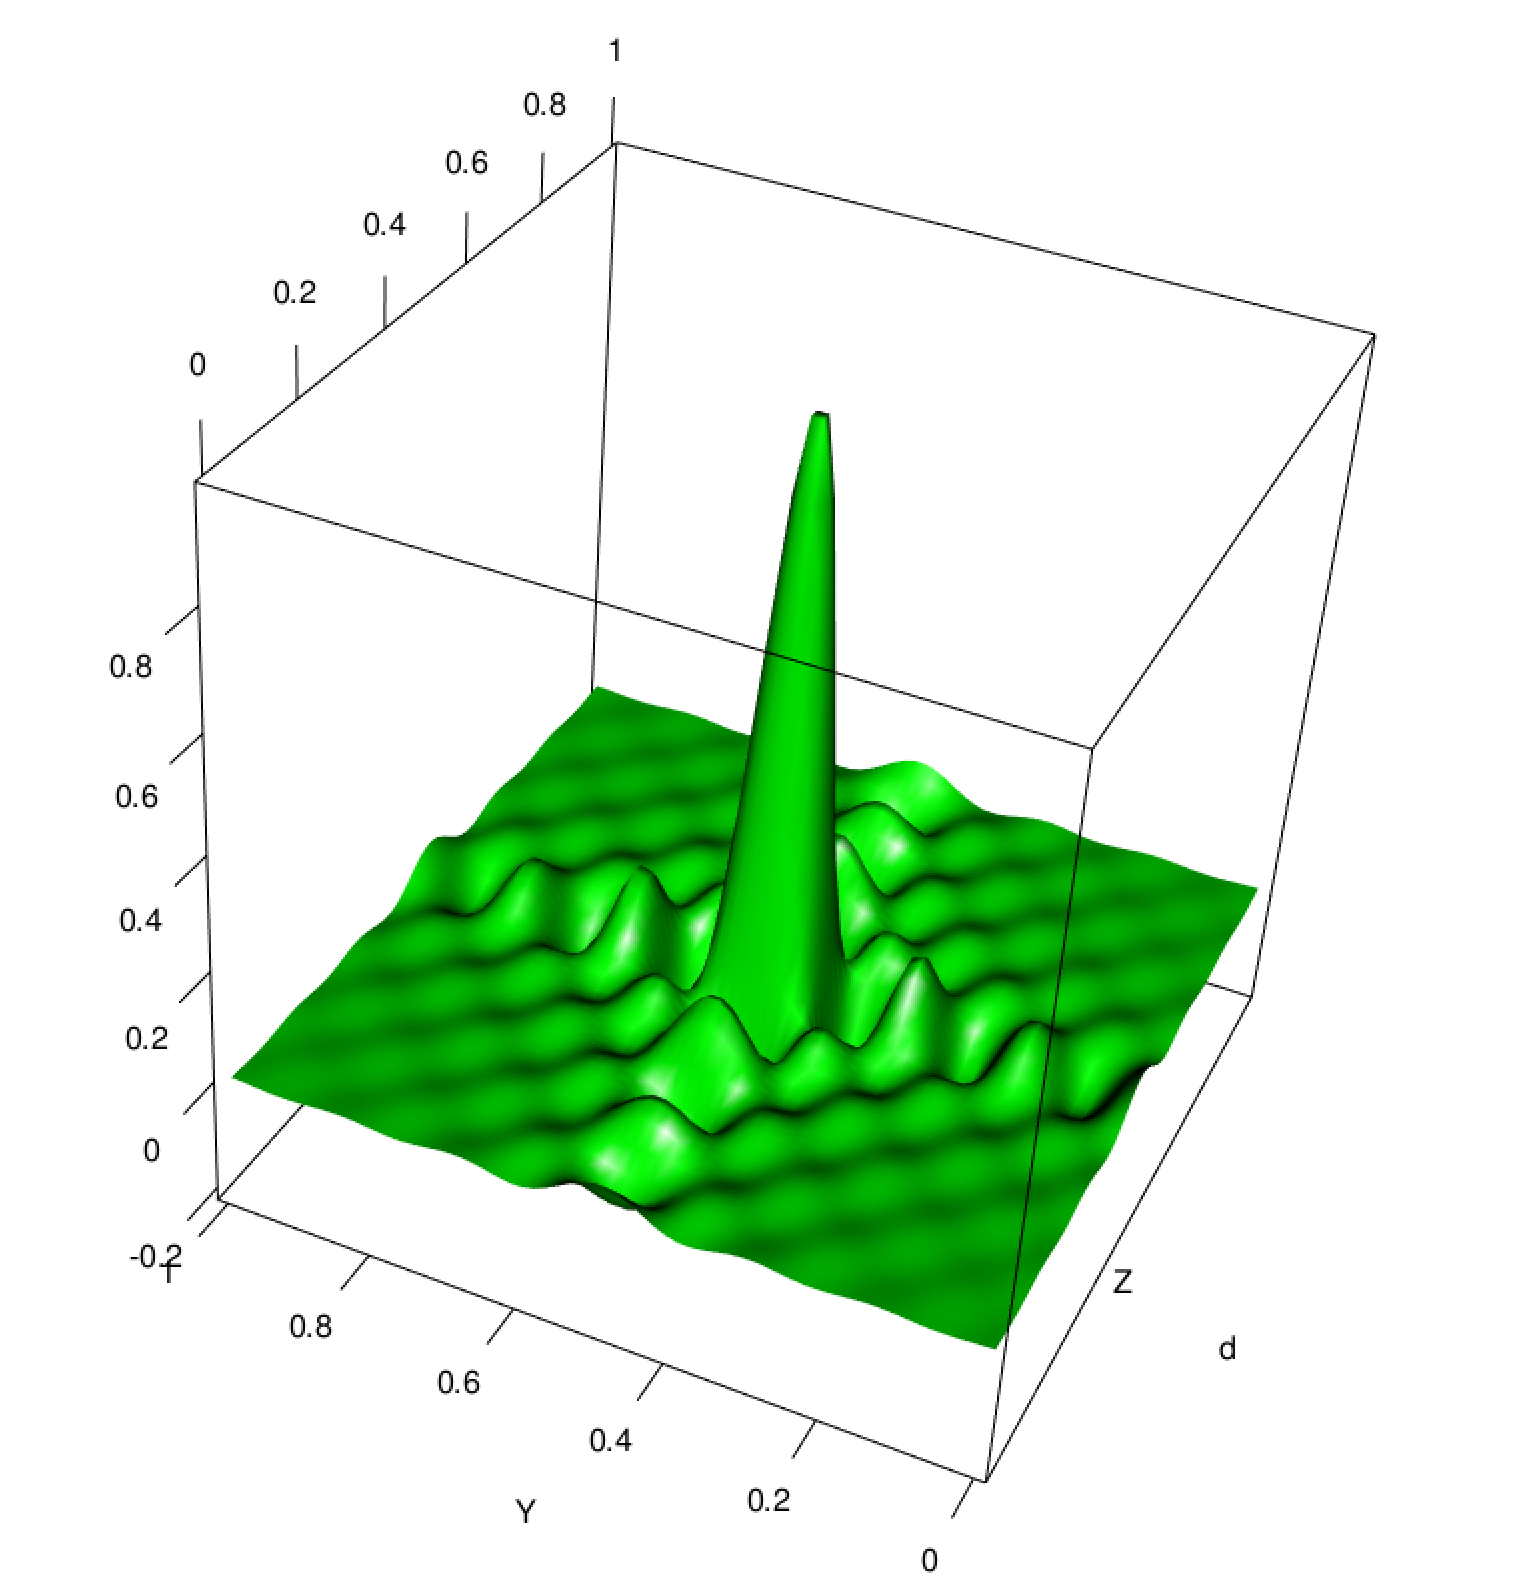
\includegraphics[width=\textwidth]{sinc_3d.png}
    \caption{
      Surface plot
    }
    \label{fig:sinc:3d}
  \end{subfigure}
  \qquad\qquad%
  \begin{subfigure}[b]{0.3\linewidth}
    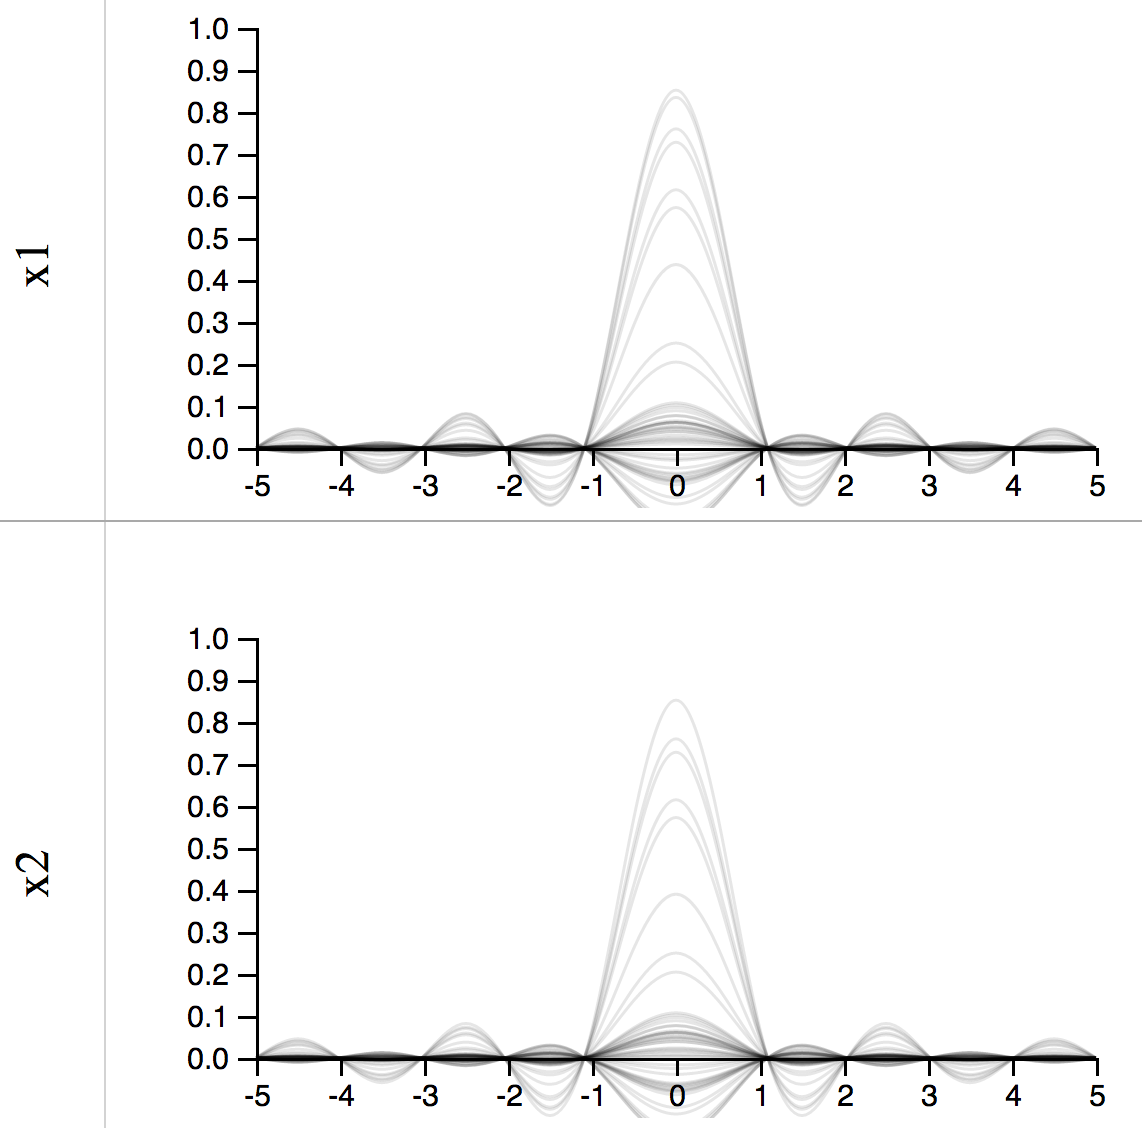
\includegraphics[width=\textwidth]{sinc_sp.png}
    \caption{
      1D slices
    }
    \label{fig:sinc:sp}
  \end{subfigure}
  \\
  \begin{subfigure}[b]{0.3\linewidth}
    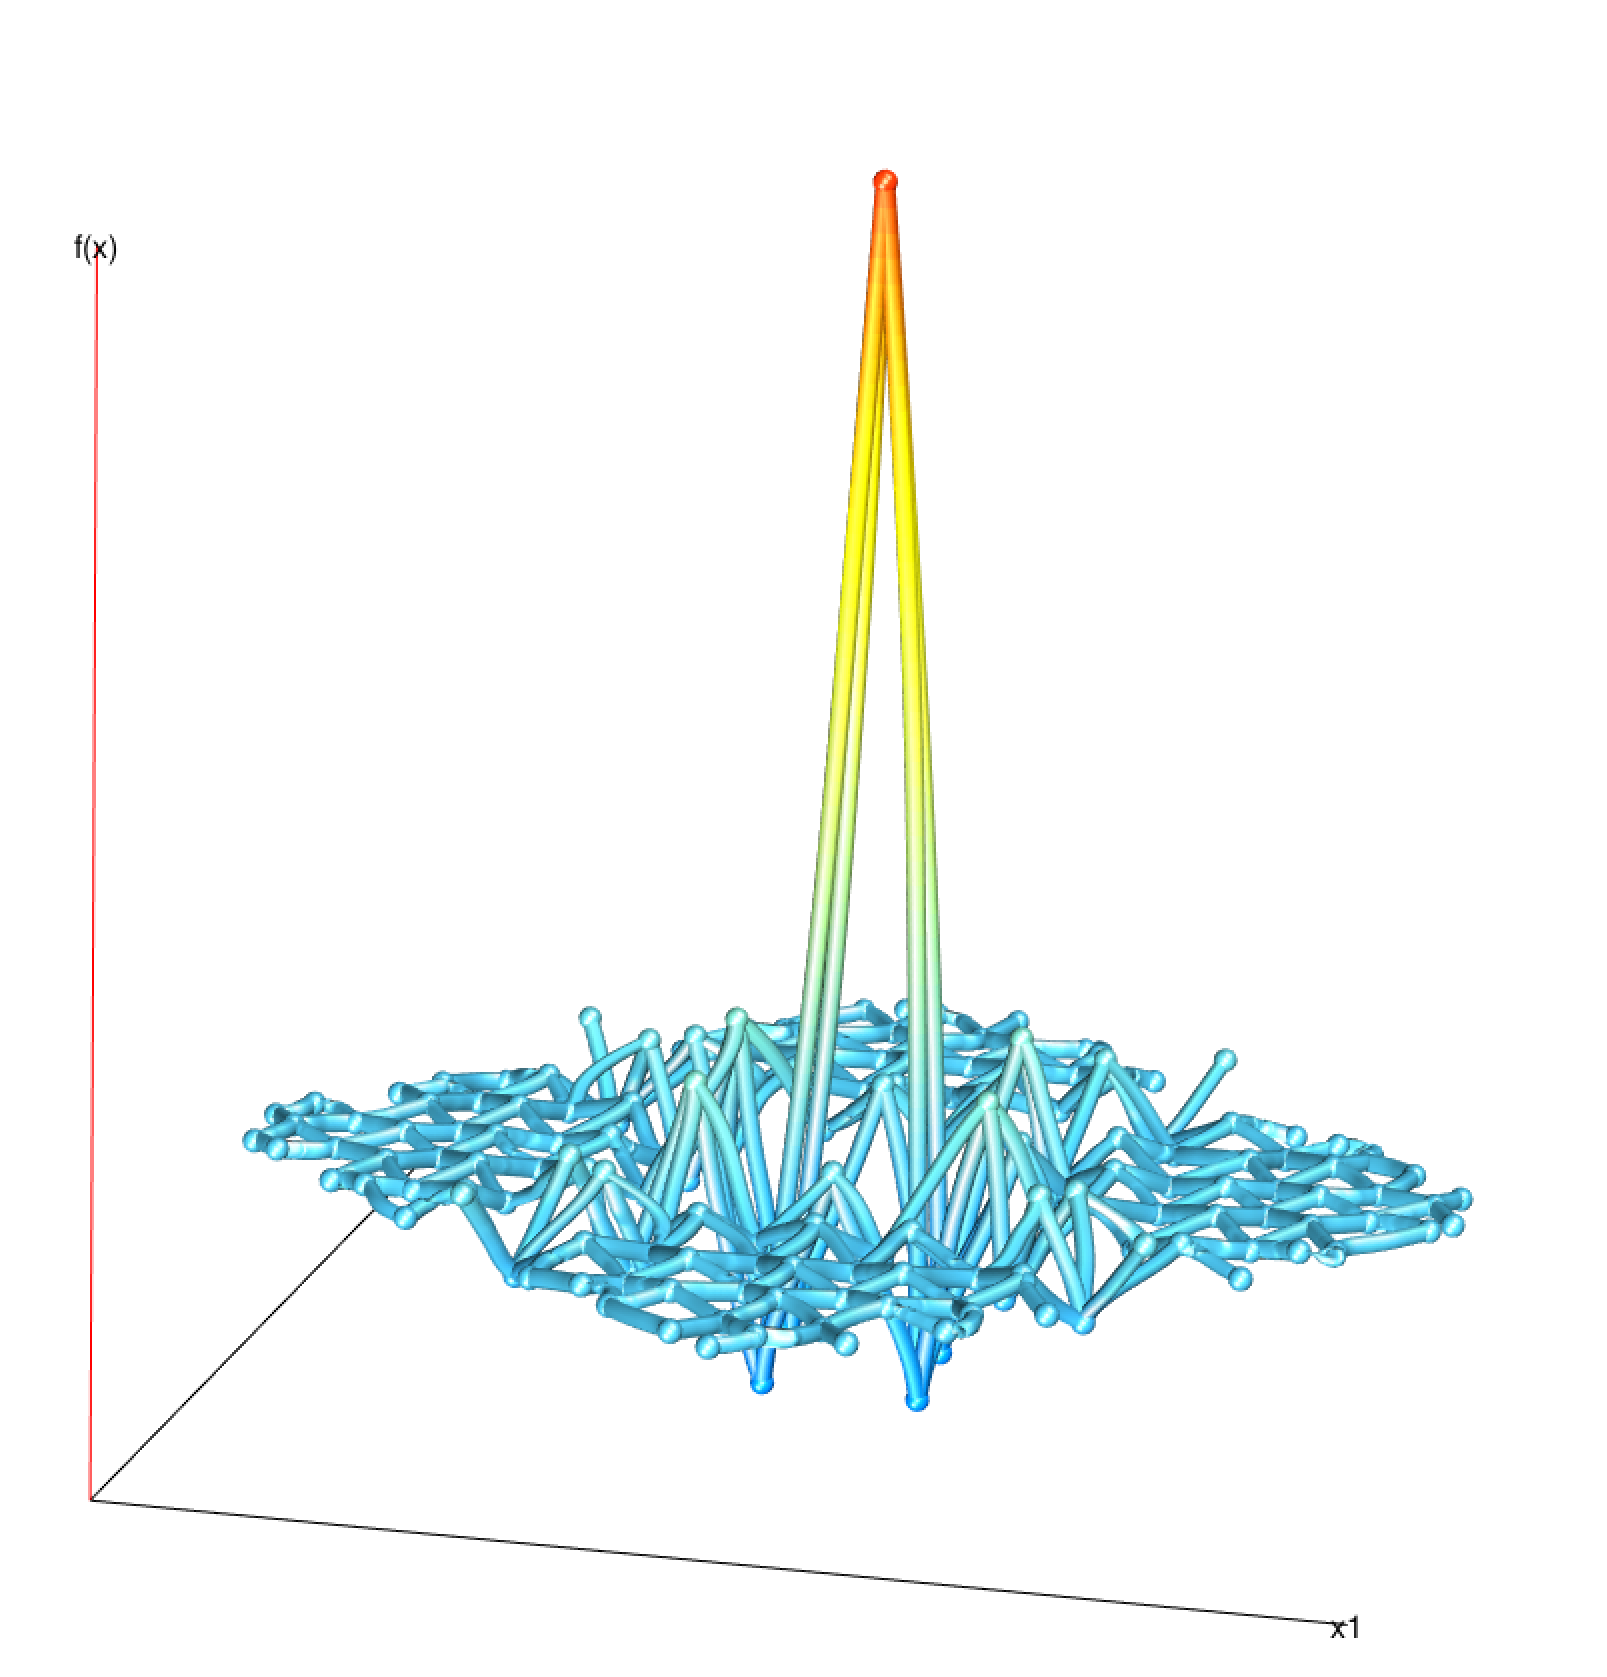
\includegraphics[width=\textwidth]{sinc_ms_1.png}
    \caption{
      $\texttt{pLevel} = 0.0$
    }
    \label{fig:sinc:ms_1}
  \end{subfigure}
  \hfill
  \begin{subfigure}[b]{0.3\linewidth}
    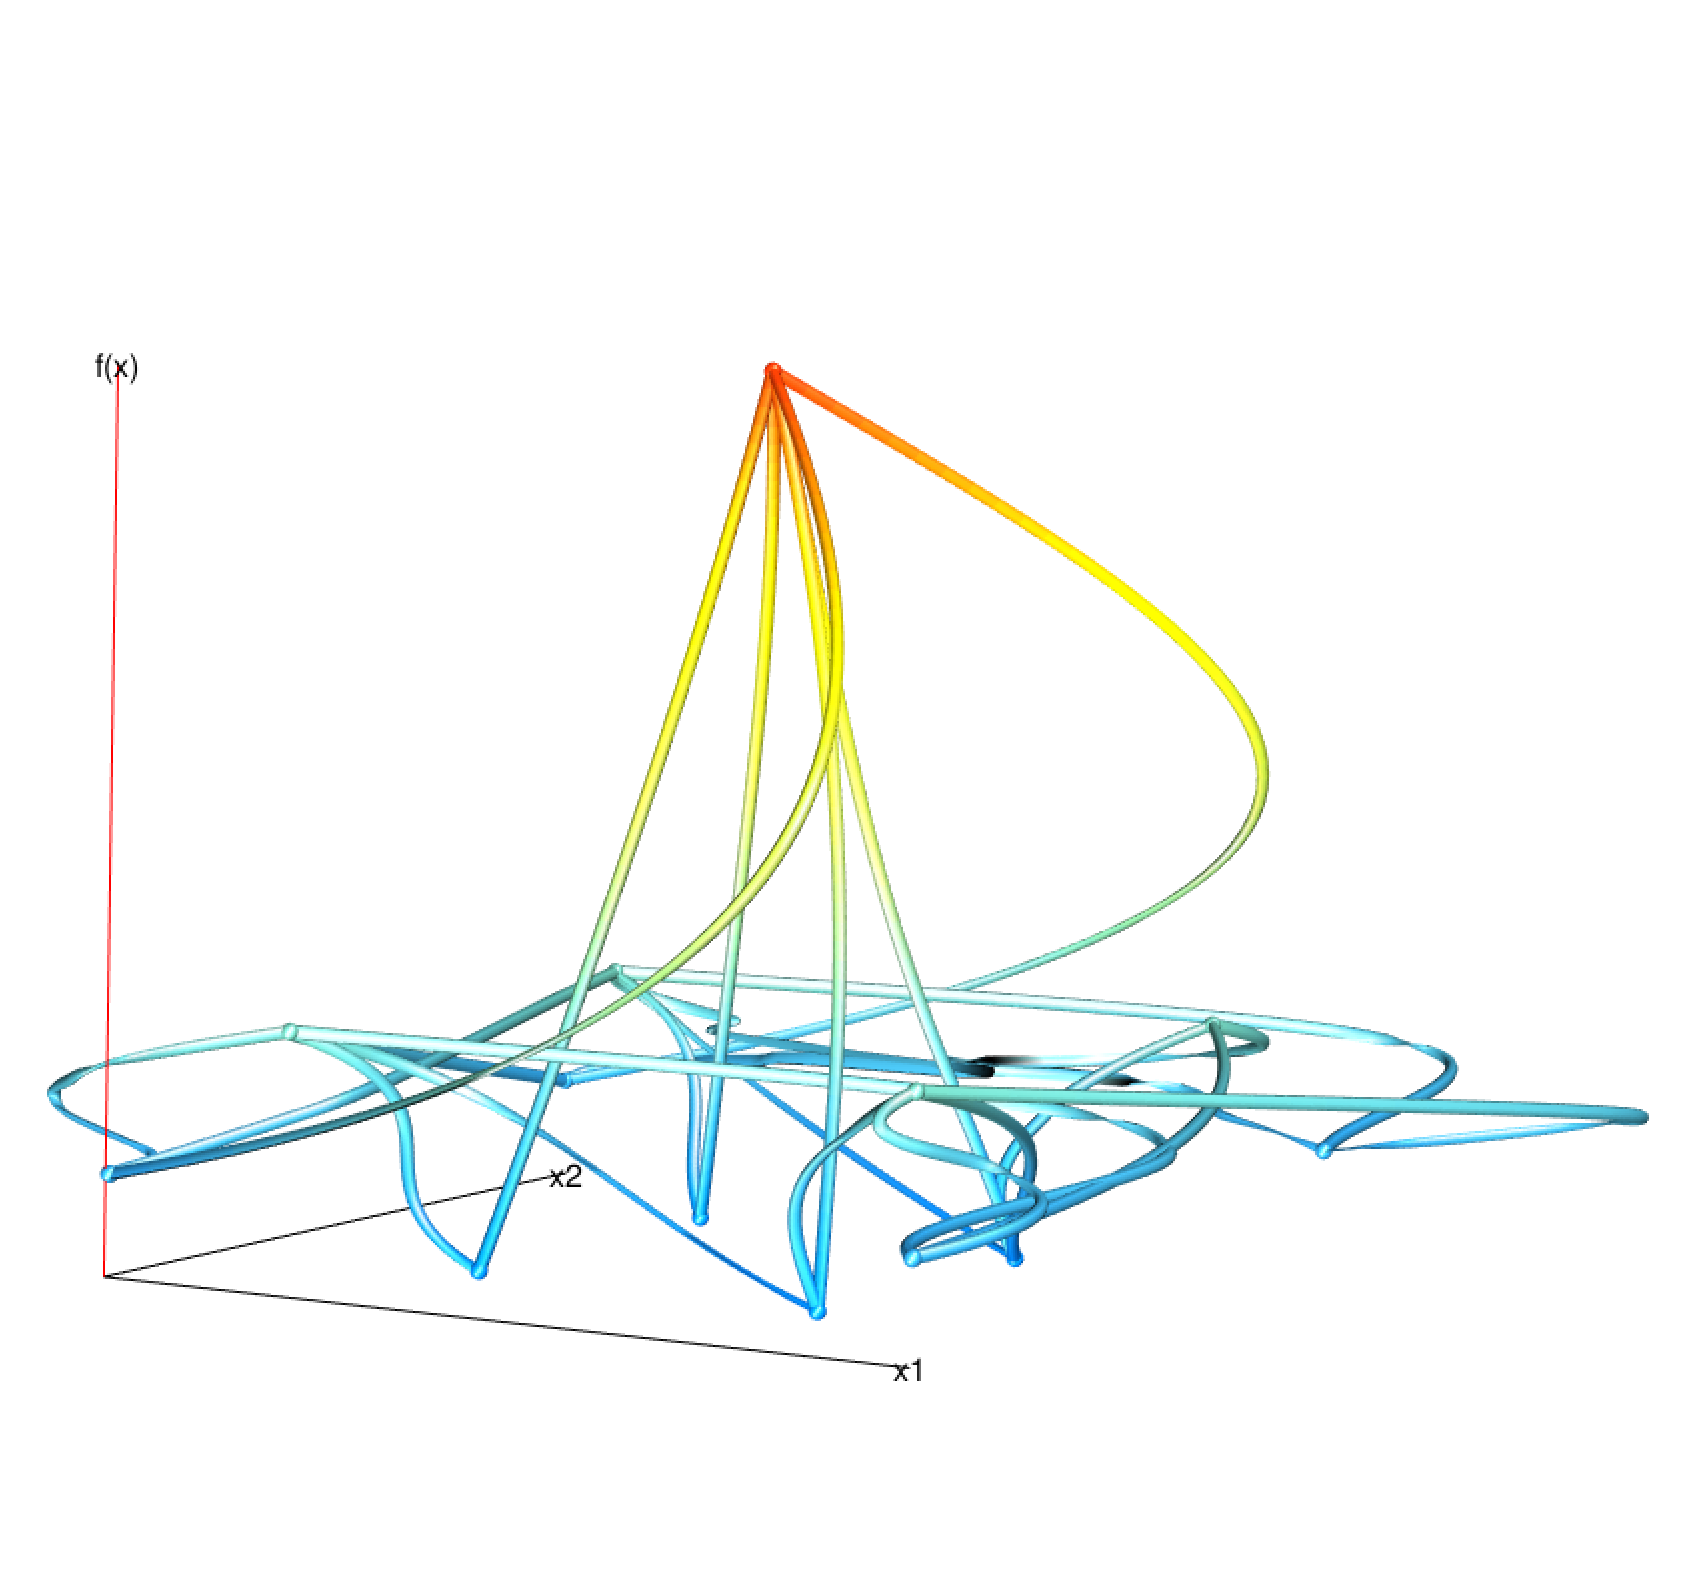
\includegraphics[width=\textwidth]{sinc_ms_2.png}
    \caption{
      $\texttt{pLevel} = 0.05$
    }
    \label{fig:sinc:ms_2}
  \end{subfigure}
  \hfill
  \begin{subfigure}[b]{0.3\linewidth}
    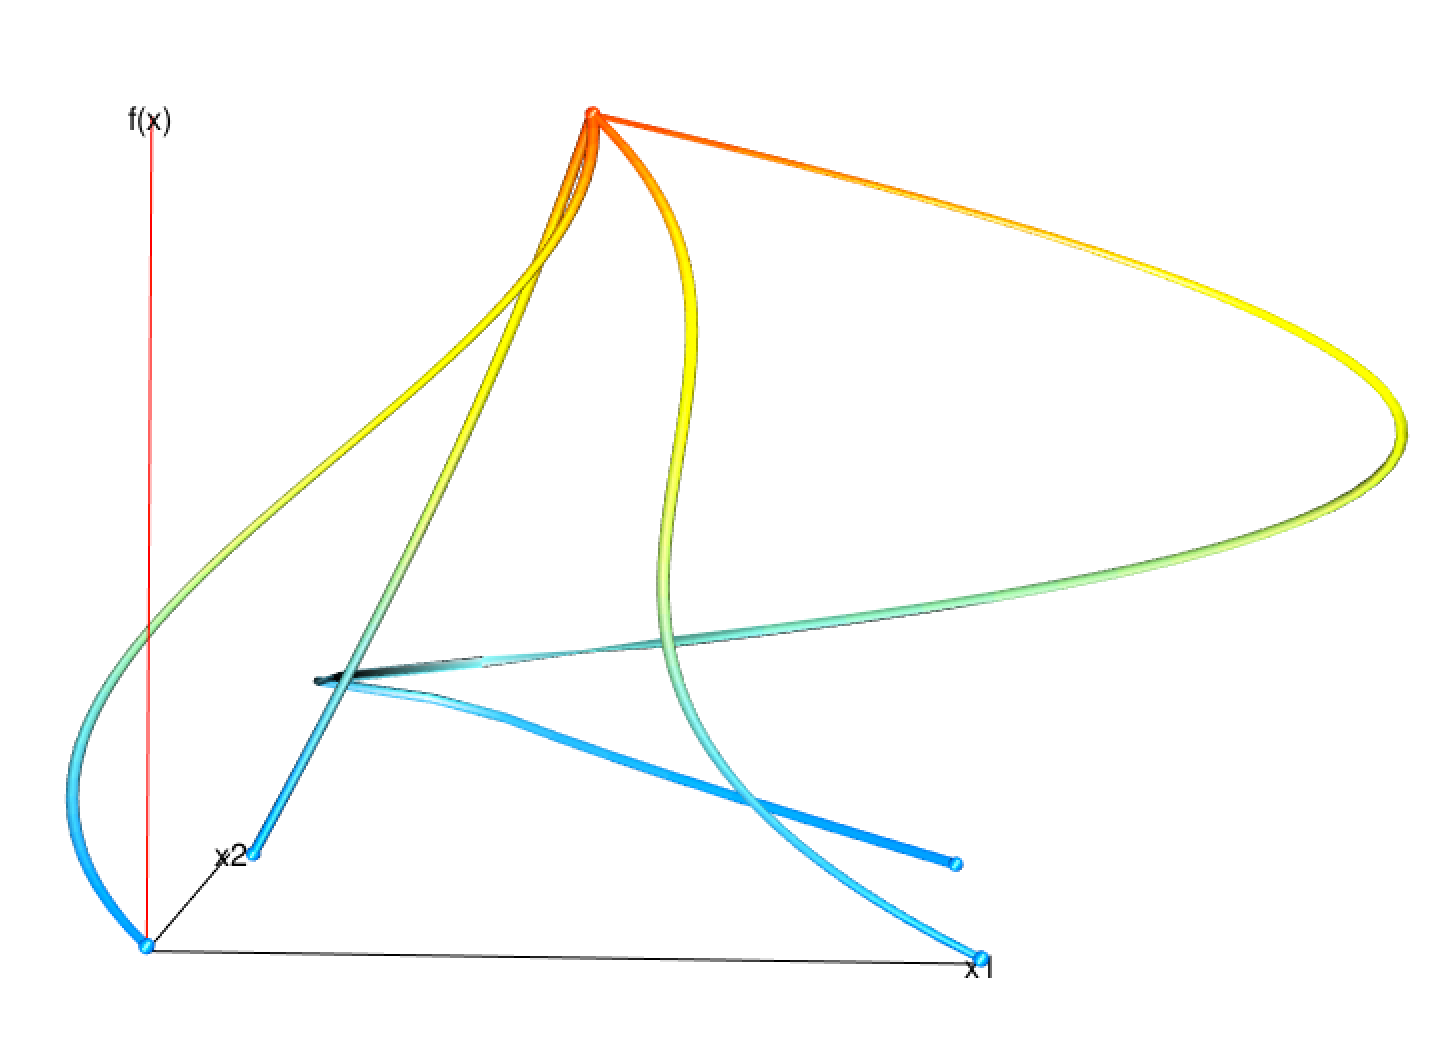
\includegraphics[width=\textwidth]{sinc_ms_3.png}
    \caption{
      $\texttt{pLevel} = 0.1$
    }
    \label{fig:sinc:ms_3}
  \end{subfigure}
  \caption{
    Different views of the 2D sinc function. We show the surface plot
    in (\subref{fig:sinc:3d}) for reference. Our 1D slice view is shown
    in (\subref{fig:sinc:sp}). The central peak as well as the sub peaks
    are prominent. For comparison we show the method of Gerber et 
    al.~\cite{Gerber:2010} in 
    (\subref{fig:sinc:ms_1})--(\subref{fig:sinc:ms_3}) at different levels 
    of persistence filtering. 
    With no filtering (\subref{fig:sinc:ms_1}) the graph looks much like the
    original function. The plot is very sensitive to the filtering level.
    (\subref{fig:sinc:ms_2}) and (\subref{fig:sinc:ms_3}) are all very 
    different from each other.
  }
  \label{fig:sinc}
\end{figure}

Imagining how a function in more than 3-dimensions looks is difficult if not
impossible. In order to illustrate how Sliceplorer visualizes functions we show
the 2D sinc function. 
%\tmnote{The sinc function is a the perfect reconstruction function in the band limited case.}
We are using the formulation where 
$y(x_1,x_2) = \frac{sin(\pi x_1)}{\pi x_1} \frac{sin(\pi x_2)}{\pi x_2}$.
In \autoref{fig:sinc:3d} we show a 3D surface plot of this function. The 
global maximum is at $x_1,x_2 = 0,0$ where $y=1$. There are a number of local
maxima and minima of decreasing value radiating out from the origin.

We show the 1D slice view using Sliceplorer in \autoref{fig:sinc:sp}.
We are showing 50 slices in each of the 2 plots. We can clearly see that
the maximum value occurs when $x_1,x_2 = 0,0$ in the graph at around $y=1$.
We can also see the decreasing extrema radiating out from the origin. We can
also precisely measure the height and x-location of the extrema. If we want
to examine a particular trace then we can highlight it in the view and see
the full slice highlighted on screen.

For comparison, we show visualizations of the 2D sinc function rendered using
the \texttt{msr} package~\cite{Gerber:2012} in R. This package implements the
visualization of the Morse-Smale complex from Gerber et al.~\cite{Gerber:2010}.
We sampled the function with $2000$ sample points using a Sobol sequence. The
1D slices view is showing $50$ focus points with $21$ samples for each slice so
this was done to use a similar sampling method and number of samples to the
Sliceplorer method. The function can do persistence-based filtering of the
graph before rendering.  This is controlled by the \texttt{pLevel} parameter
which filters all persistences less than a certain value. In
\autoref{fig:sinc:ms_1} we show the view with the filtering level set to $0$,
i.e.\ no filtering. The view does a very good job showing the critical points
of the graph. It looks very similar to the surface plot
(\autoref{fig:sinc:3d}). However, the visualization is very sensitive to the
filtering level. In \autoref{fig:sinc:ms_2} and \autoref{fig:sinc:ms_3} we show
the sinc function with the filtering level set to $0.05$ and $0.1$
respectively.  The 1D slice view does not suffer from this issue of
parameterization.

\subsection{Neural networks}\label{neural-networks}

\begin{figure*}[t]
  \centering
  \begin{tabular}[b]{cccc}
    Neural network - 26 & SVM - polynomial & Neural network 5+3 & SVM - radial \\
    \hline \\
    \begin{subfigure}[b]{0.2\textwidth}
      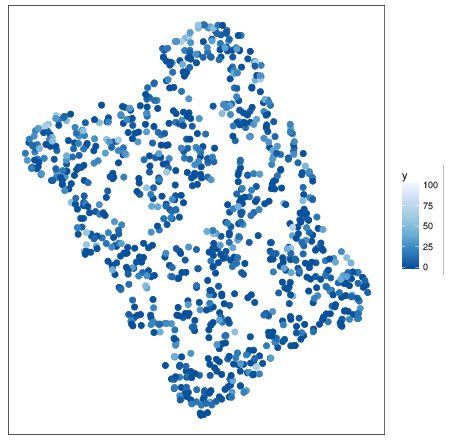
\includegraphics[width=\textwidth]{boston_nn_26_sp.png}
      \caption{
      }
      \label{fig:nn_comp:a}
    \end{subfigure}
    &
    \begin{subfigure}[b]{0.2\textwidth}
      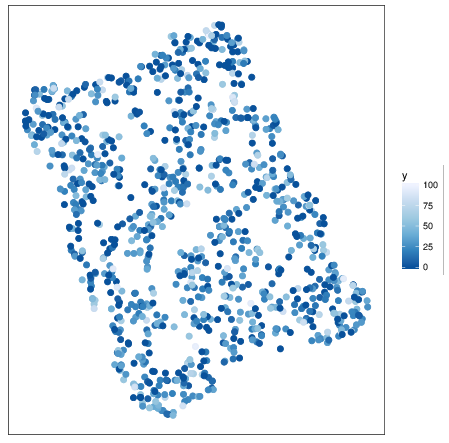
\includegraphics[width=\textwidth]{boston_svm_poly_sp.png}
      \caption{
      }
      \label{fig:nn_comp:b}
    \end{subfigure}
    &
    \begin{subfigure}[b]{0.2\textwidth}
      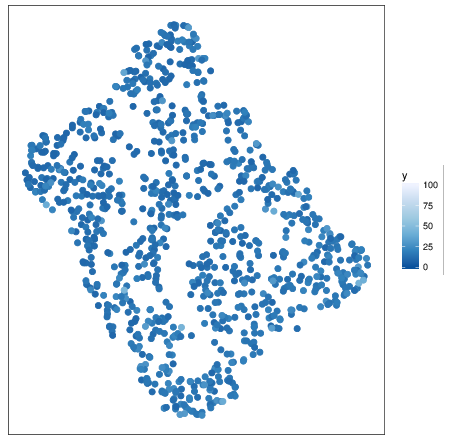
\includegraphics[width=\textwidth]{boston_nn_5x3_sp.png}
      \caption{
      }
      \label{fig:nn_comp:c}
    \end{subfigure}
    &
    \begin{subfigure}[b]{0.2\textwidth}
      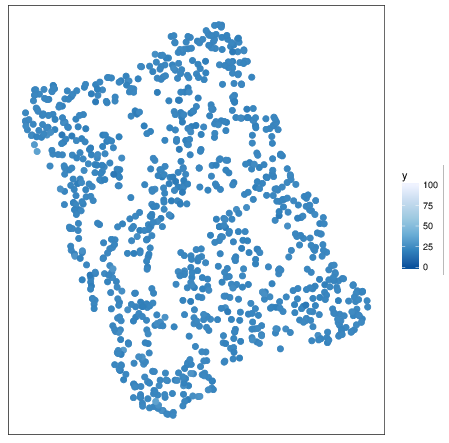
\includegraphics[width=\textwidth]{boston_svm_radial_sp.png}
      \caption{
      }
      \label{fig:nn_comp:d}
    \end{subfigure} \\
    \begin{subfigure}[b]{0.2\textwidth}
      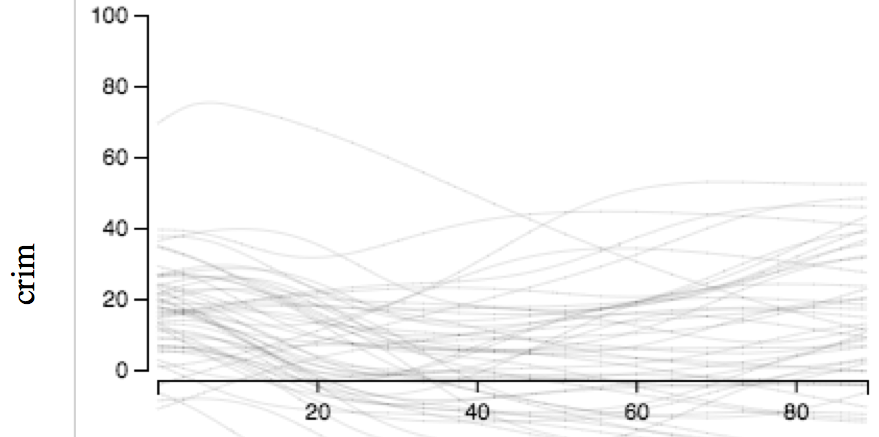
\includegraphics[width=\textwidth]{boston_nn_26_slices.png}
      \caption{
      }
      \label{fig:nn_slices:e}
    \end{subfigure}
    &
    \begin{subfigure}[b]{0.2\textwidth}
      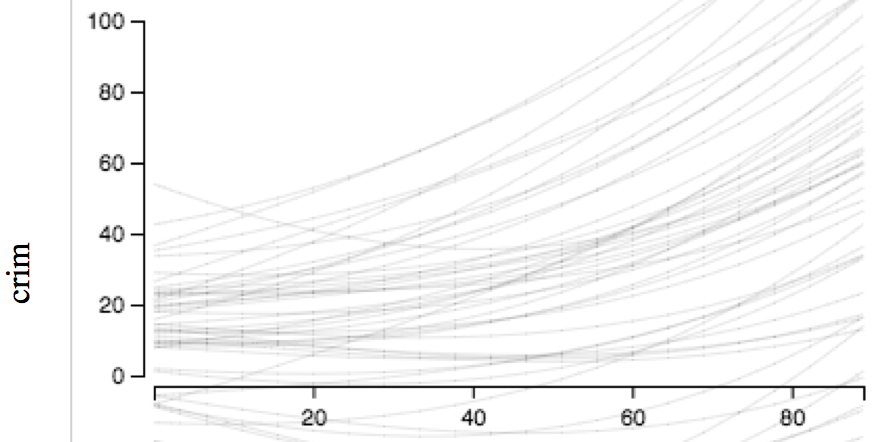
\includegraphics[width=\textwidth]{boston_svm_poly_slices.png}
      \caption{
      }
      \label{fig:nn_slices:f}
    \end{subfigure}
    &
    \begin{subfigure}[b]{0.2\textwidth}
      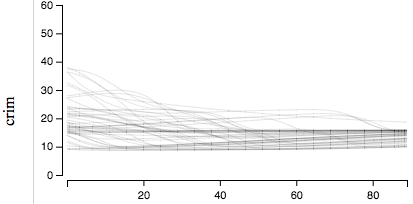
\includegraphics[width=\textwidth]{boston_nn_5x3_slices_zoomed.png}
      \caption{
      }
      \label{fig:nn_slices:g}
    \end{subfigure}
    &
    \begin{subfigure}[b]{0.2\textwidth}
      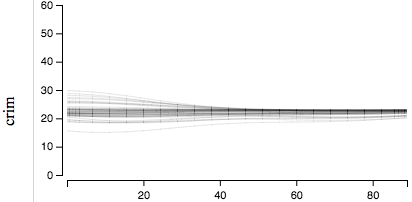
\includegraphics[width=\textwidth]{boston_svm_radial_slices_zoomed.png}
      \caption{
      }
      \label{fig:nn_slices:h}
    \end{subfigure}
  \end{tabular}
  \caption{
    Two different views of the predictions of four different machine learning
    regression models on the Boston housing dataset. The top row (a -- d) shows
    predictions by each model compressed to two dimensions with t-SNE. We
    colored the points on a continuous color scale with dark blue being 0 and
    light blue the highest value. The bottom row (e -- h) shows a 1D slice view
    of the first dimension of the dataset, crime rate. We show the slices of
    the remaining dimensions in the supplemental material. 
    The 1D slices reveal interesting information about how the models perform and
    can assist with model selection. We may not want to use the SVM with
    polynomial kernel (f), for example, since it predicts that home price will go
    up with higher crime rates.
  }
  \label{fig:nn_comp}
\end{figure*}

%\msnote{sounds a bit too defensive. Deep Learning is the big hype at the moment but nobody understands them! That's imho the core message that we need to say}
Artificial neural networks are currently gaining a lot of attention in machine
learning.  The goal of these algorithms is to produce a multi-dimensional
function fitted to the training points. Neural networks, in particular, have
proven to be very good at producing accurate, generalizable predictions. One of
the major challenges for designers of such models, however, is to properly
architect these networks. For instance, how many hidden layers does one need
and how many nodes should be put into each layer? These architectural choices
can drastically change the predictions.
While these choices are crucial, currently, there is only
little guidance available for designers. A typical rule of thumb is to
use a hidden layer two times the size of the input dimensions.
% or two layers with \ttwnote{some reduction}. 
There are also some general proofs regarding what type of functions neural
networks can represent~\cite{Hornik:1989,Eldan:2016}. However, there are no
formal guidelines for designing these networks~\cite{Goodfellow:2016} and the
way these models make predictions is still obtuse.

One of the ways we can increase the understandability of neural network
regression models is by viewing the response function
directly~\cite{gleicher:2016}. If we want to understand how the network
architecture affects the prediction we could compare the prediction manifold to
one produced by a ``simpler'' machine learning model~\cite{Ribeiro:2016a}, for
example a support vector machine~\cite{Smola:2004}.  Support vector machines
have known guarantees on error rate with the number of training samples. With
this comparison we may be able to get some better insight about how the neural
network learning algorithms are performing.

To compare, we chose the Boston housing dataset~\cite{Lichman:2013} from the
UCI repository. This dataset contains median home prices
given 13 factors including crime rate, age of the house, and proximity to
highways. We then trained a neural network with a single hidden layer of 26
nodes, a neural network with 2 hidden layers: one of 5 and one of 3 nodes, a
support vector machine with a polynomial kernel, and a support vector machine
with a radial (Gaussian) kernel.
%\msnote{Ok, add more detailed notes ... I think the challenge is to add a
%couple of subclauses explaining the ML background in a nutshell and connect it
%to / make its relevance for the problem at hand clear (abstractly, we would
%like to look at and understand multi-D respose surfaces, i.e. multi-D
%continuous functions. As soon as we can see these functions, we also can
%compare different models. That is, if models have similar response surface
%functions, we can use the easier to understand one to as a ``surrogate'' to
%better understand the behavior of the more complex ones ... just some thoughts
%in my words, not sure if this is actually what we want to achieve, but our
%goals should be very clear here ... Said all that, to me I think it is mostly
%clear what you mean, but I might be biased here as I do know our project well
%and can fit in all the pieces without any problem.  ... old: for the above
%paragraphs: need to be explained more clearly imho.  Specifically, they should
%also make the issues and concepts clear to someone who is not necessarily an
%ML expert. Needs re-writing; happy to discuss to give some ideas on what a
%good level of information would be here.}

We compare 1D slices with an adaption of the common way of viewing
classification algorithms to continuous data.
% to maintain \ttwnote{ecological validity?}. 
The results of \emph{classification} models are commonly visualized
by using MDS~\cite{Kruskal:1964} or t-SNE~\cite{Maaten:2008} to reduce the input
dimensions to two and then present a scatterplot with the predictions colored
by class. We extended this by sampling the prediction model with \(1,000\)
samples from a Latin hypercube~\cite{Tang:1993} (a space-filling design)
converting the points to two dimensions with t-SNE and then coloring the points
on a continuous scale which we show in \autoref{fig:nn_comp} (top row).  The
bottom row of the figure shows the 1D slice view of the same four prediction
models. We only show the first dimension due to space reasons. The full 13
dimension slice view image is in the supplemental material.

Showing the changes in home price as it corresponds directly to the crime rate
can help to increase confidence in a model.  From the prediction lines, one may
not want to use the SVM with a polynomial kernel. By and large the prediction
lines are increasing. This means that the home price is increasing as the crime
rate goes up. This does not really make sense. The model is not generalizing
well. Similarly, the neural network with a single hidden layer (left column)
also has a number of curves that increase as crime increases. The neural
network with two hidden layers does not have this problem. Maybe this is the
best model to use in this case.

%\tmnote{needs a final paragraph, maybe sth like} 
In summary, this usage scenario illustrated that a direct inspection of a
model's response surfaces can give intuition of its behavior, and can lead to a
better model selection and a better intuition of the modeling process. 1D
slices can help to gain important insights in this process. 
%Hence, this type of analysis is not only novel but also insightful.

\subsection{Optimization algorithm}
\label{sec:optimization}

General purpose optimization algorithms try to find the global minimum (or
equivalently, the global maximum) of a function of arbitrary dimension.  Many
optimization algorithms such as Nelder-Mead~\cite{Nelder:1965} work by starting
at a particular parameter setting and evaluating the ``shape'' of the function
around that point.  The algorithm then determines where the function is
decreasing the greatest, and ``jumps'' a certain distance in that direction.
The ``jump'', starting position, and termination tolerance parameters are
user-settable parameters. Depending on how they are set, the algorithm can get
stuck in a local minima or take unreasonably long to finish.

When one is trying to parameterize or build optimization algorithms then
one wants to evaluate the trace of the optimization on an easy function
that is fast to compute first. This analysis helps to better understand how to parameterize for more complex problems
%, which will be faced in reality, 
but are
too computationally expensive to analyze directly. 
Visual inspection of the easy function before running the optimization algorithm, as well as
viewing the trace of the optimization algorithm (the sequence of steps it took) is a good way to ensure that the algorithm is converging towards the global
minimum. 
%\msnote{... maybe something: you would also like to use the algorithm
%inn other situations as well or so?}\ttwnote{not sure what you mean}
%\msnote{... old: just playing devil's advocate: So, we have the visual minimum,
%why care about the visualization then if you simply could compute a number
%between the visual global minimum and the algorithmically detected minimum}
%\msnote{TO DISCUSS: what about a number for the difference between the visual minimum in the slices and 
%the local minimum found?}
%\msnote{TO DISCUSS: also, how would the other alternatives perform here?}

We compare 1D slices with HyperSlice~\cite{Wijk:1993} as this is the only
technique that also directly visualizes the parameter space.  We ran the
Nelder-Mead optimization algorithm on the 5D Ackley
function~\cite{Ackley:1987}, a popular optimization algorithm testing function.
To examine the effect of starting position, we tried different starting
positions: \(x=(1,1,1,1,1)\) and \(x=(2,2,2,2,2)\).  We overlay the
optimization trace on top of both 1D slices and HyperSlice and the results are
shown in \autoref{fig:optim_trace}.

\begin{figure}
  \centering
  \begin{subfigure}[b]{0.35\linewidth}
    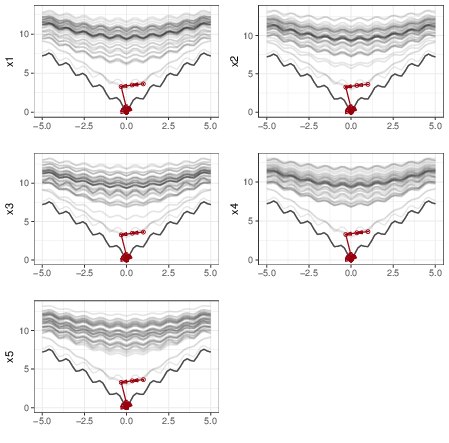
\includegraphics[width=\textwidth]{optim_trace_1_1.png}
    \subcaption{ 
      \label{fig:optim_1:sp}
    }
  \end{subfigure}
  \qquad\qquad
  \begin{subfigure}[b]{0.35\linewidth}
    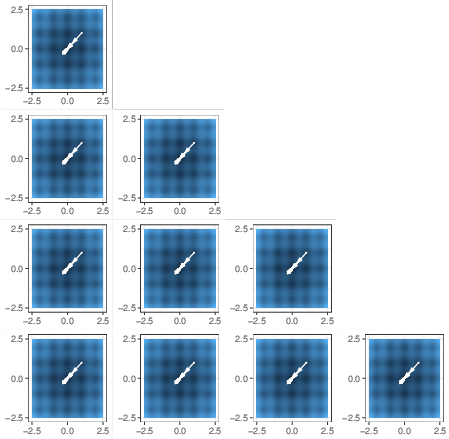
\includegraphics[width=\textwidth]{optim_trace_hs_1_1.png}
    %\resizebox{\textwidth}{!}{%
    %\begin{tabular}{rrrrr}
      %20.9885770  & -0.3256642 & -0.3257547 & -0.3258958 & -0.3252083 \\
      %-0.3256642  & 20.9908910 & -0.3254367 & -0.3255775 & -0.3248914 \\
      %-0.3257547  & -0.3254367 & 20.9902343 & -0.3256679 & -0.3249814 \\
      %-0.3258958  & -0.3255775 & -0.3256679 & 20.9892087 & -0.3251219 \\
      %-0.3252083 & -0.3248914 & -0.3249814 & -0.3251219 & 20.9941950
    %\end{tabular}
    %}
    \subcaption{
      \label{fig:optim_1:hs}
    }
  \end{subfigure}
  \\
  \begin{subfigure}[b]{0.35\linewidth}
    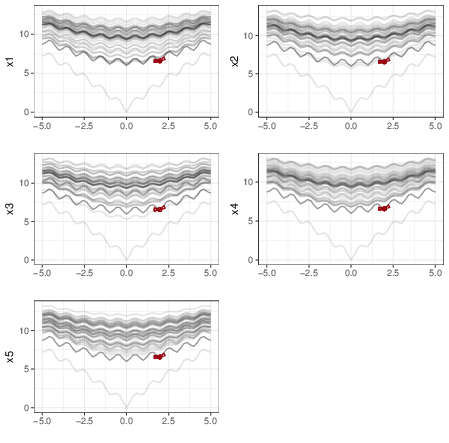
\includegraphics[width=\textwidth]{optim_trace_2_1.png}
    \subcaption{
      \label{fig:optim_2:sp}
    }
  \end{subfigure}
  \qquad\qquad
  \begin{subfigure}[b]{0.35\linewidth}
    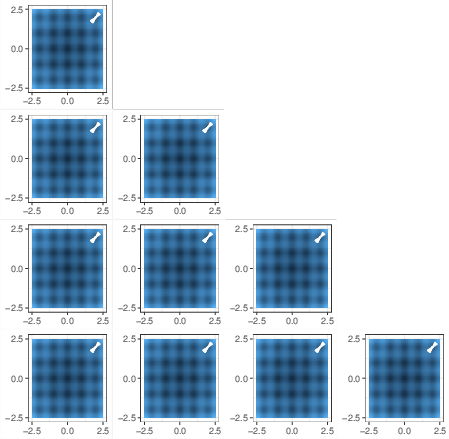
\includegraphics[width=\textwidth]{optim_trace_hs_2_1.png}
    %\resizebox{\textwidth}{!}{%
    %\begin{tabular}{rrrrr}
      %21.0042955 & -0.1840739 & -0.1843067 & -0.1846840 & -0.1845613 \\
      %-0.1840739 & 21.0067633 & -0.1839595 & -0.1843355 & -0.1842132 \\
      %-0.1843067 & -0.1839595 & 21.0051112 & -0.1845689 & -0.1844464 \\
      %-0.1846840 & -0.1843355 & -0.1845689 & 21.0024265 & -0.1848241 \\
      %-0.1845613 & -0.1842132 & -0.1844464 & -0.1848241 & 21.0033008
    %\end{tabular}
    %}
    \subcaption{
      \label{fig:optim_2:hs}
    }
  \end{subfigure}
  \caption{
    1D slice and HyperSlice views showing
    traces of an optimization algorithm searching for the global minimum
    of a 5D Ackley function.
    (\subref{fig:optim_1:sp}) and 
    (\subref{fig:optim_1:hs}) show the trace starting at the point
    $(1,1,1,1,1)$ while 
    (\subref{fig:optim_2:sp}) and 
    (\subref{fig:optim_2:hs}) 
    show the trace starting at the point $(2,2,2,2,2)$. 
  }
  \label{fig:optim_trace}
\end{figure}

The 1D slice view allows us to see the path that the algorithm took and the
general shape of the function simultaneously.  In addition, the 1D slice view
shows that the distribution of values around the global minimum is small. Most
of the slices are clustered around \(y=10\) with only one slice descending
close to \(y=0\). Since the sampling is uniform in the parameter space this
means that it is very difficult to select slices around the global minimum. In
fact, this is a known property of the Ackley function.  It is easy to see that
the optimization algorithm got stuck at a local minimum when started at
\(x=(2,2,2,2,2)\). However, with the HyperSlice view it is difficult to see the
difference in value and steepness of the function at \(x=(1,1,1,1,1)\) versus
\(x=(2,2,2,2,2)\).  Humans are not good at perceiving fine differences in
color~\cite{Munzner:2014}, but is required for this task. We learn a lot more
about the behavior of the optimization algorithm from the 1D slice views (see
\autoref{fig:optim_1:sp} and \autoref{fig:optim_2:sp}) than the HyperSlice
view. However, the HyperSlice view does clearly show that that optimization
algorithm is moving in multiple directions at once. This is not clear in the 1D
slice views.


